\newpage
\section{Exception Handling}
	Abnormale aber vorhersebare und m�gliche Bedingung bei der Programmausf�hrung.\\
	\begin{minipage}[t]{11cm}
		\subsection{Handling Strategie von System Exceptions}
			\begin{compactitem}
				\item In \lc{Java} und \lc{C\#} gelangen die System Exceptions in die Sprache, d.h. eine LowLevel Exception wird in eine Exception der Programmiersprache gemappt.
				\item Die Sprache \lc{C++} betreibt kein solches Exception Mapping, d.h. Low-Level 
				Exceptions werden nicht von \lc{C++} geworfen und k�nnen auch nicht mit
				\lc{catch(...)} abgefangen werden.
				\item Der Hauptgrund daf�r ist einmal mehr Effizienz. Wenn st�ndig Exceptions
				herumfliegen (auch wenn sie nicht abgefangen werden), dann beeintr�chtigt
				das die Performance.
				\item Einzelne Systemumgebungen betreiben dennoch Exception Mapping in \lc{C++}
				(z.B. \lc{Microsoft} in \lc{Visual C++}).
			\end{compactitem}
	\end{minipage}
	\hspace*{0.5cm}
	\begin{minipage}[t]{7cm}
		\subsection{Ziel}
		\begin{compactitem}
			\item Der Normalfall soll einfach gelesen werden k�nnen
			\item Der Ausnahmefall ist klar und einfach geregelt
			\item Der Overhead soll m�glichst klein sein
			\item Die Weiterreichung an die n�chsth�here Funktion im Call Stack soll einfach sein
		\end{compactitem}
	\end{minipage}

	\subsection{Exceptionhandling in \lc{C++}}
	\begin{compactitem}
		\item Exceptions werden in Form eines Objekts am Ort ihres Auftretens ausgeworfen (explizit oder auch "automatisch").
		\item Exception Handler versuchen, diese Exception-Objekte aufzufangen.
	\end{compactitem}

	\begin{minipage}[t]{9 cm}
		\subsubsection{Ausl�sen (Werfen) von Ausnahmen}
			\begin{compactitem}
				\item Ausnahmen k�nnen mit dem Schl�sselwort \lc{throw} explizit ausgeworfen werden.
				\item Nach einem \lc{throw}-Befehl wird das Programm abgebrochen und beim ersten passenden umgebenden Handler fortgesetzt.
				\item Dabei werden alle lokalen Objekte wieder automatisch zerst�rt (Stack unwinding).
				\item Geworfen werden kann ein beliebiges Objekt (�blich: ein spezifisches \lc{C++}-Ausnahmeobjekt).
				\item (Ausschliesslich) innerhalb eines Exception Handlers ist auch die Form
				\lc{throw;} erlaubt. Dadurch wird die Exception an den	n�chsten Handler weitergereicht (Exception propagation).
			\end{compactitem}	
	\end{minipage}
	\hspace*{0.5cm}
	\begin{minipage}[t]{9 cm}
		\subsubsection{Syntax}
			\lstinputlisting[language=C++,tabsize=2]{code/exception_handling.cpp}
	\end{minipage}
	\\
	
	\begin{minipage}[t]{11 cm}
		\subsubsection{Exception-Hierarchie in \lc{C++} und ihre Headers}		 	
			Ausnahmeobjekte k�nnen beliebigen Typs sein (z.B. auch \lc{int}). Meist werden jedoch spezifische hierarchisch organisierte Ausnahmeklassen verwendet.\\
			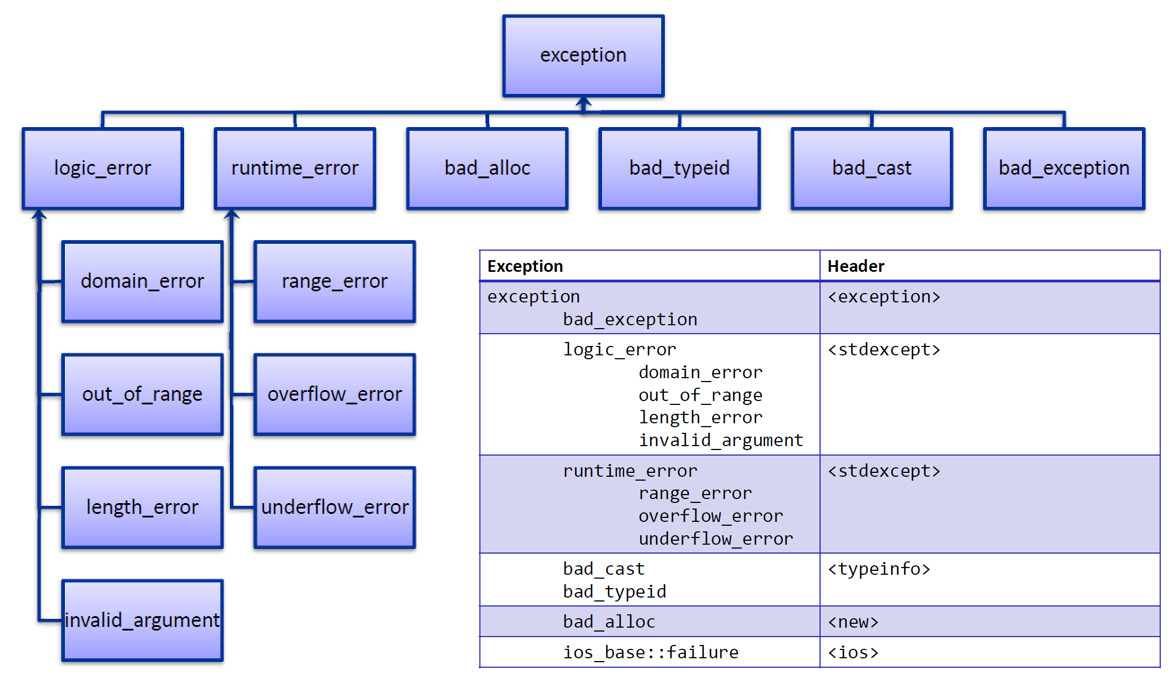
\includegraphics[width=1\textwidth]{pics/exception_hierarchy.png}
	\end{minipage}
	\hspace*{0.5cm}
	\begin{minipage}[t]{7 cm}
		\subsubsection{Laufzeit- vs. Logische Fehler}
			\begin{compactitem}
				\item Logische "Fehler" (logic\_error)
				\begin{compactitem}
					\item Ausnahmen im Programmablauf, die bereits zur Entwicklungszeit ihre Ursache	haben.
					\item Theoretisch k�nnten diese Ausnahmen verhindert werden.
				\end{compactitem}
				\item Laufzeit "Fehler" (runtime\_error)
				\begin{compactitem}
					\item Nicht vorhersehbare Ausnahmen wie z.B. arithmetische �berl�ufe.
					\item Diese Ausnahmen treten erst zur Laufzeit auf, z.B. durch eine nicht erlaubte Benutzereingabe.
				\end{compactitem}
			\end{compactitem}
	\end{minipage}
	
	%\begin{minipage}[t]{9 cm}
	\newpage
		\subsubsection{Mehrere Catches}
			\begin{compactitem}
				\item Ein oder mehrere Exception Handler k�nnen hintereinander definiert werden.
				\item Die einzelnen \lc{catch}-Handler m�ssen sich in den Parametern unterscheiden.
				\item Wenn eine Exception geflogen kommt, wird der erste passende Handler
				genommen. Ein passender Handler macht ein \lc{catch} auf genau diese Exception oder auf eine Basisklasse derselben.
				\item Deshalb (sehr wichtig): Der allgemeinste Handler (am meisten oben in der Hierarchie) muss als letzter definiert werden.
				\item Wenn kein Handler passt, dann wird im Aufrufstack nach oben gesucht, ob ein	passender Handler vorhanden ist.
				\item Wenn auch dort keiner gefunden wird, dann wird die Funktion \lc{terminate()} aufgerufen.
				\item \lc{terminate()} beendet das Programm, kann aber auch selbst definiert werden.
				\item Catch all: Der folgende Handler f�ngt ausnahmslos alle Exceptions ab (und muss wenn gew�nscht deshalb immer als letzter aufgef�hrt werden):	
			\end{compactitem}
			
			\hspace*{0.8cm}
			\begin{minipage}[t]{4cm}
				\lstinputlisting{code/catch_all.cpp}
			\end{minipage}
			\hspace*{3cm}
			\begin{minipage}[t]{10cm}
				\vspace*{-0.3cm}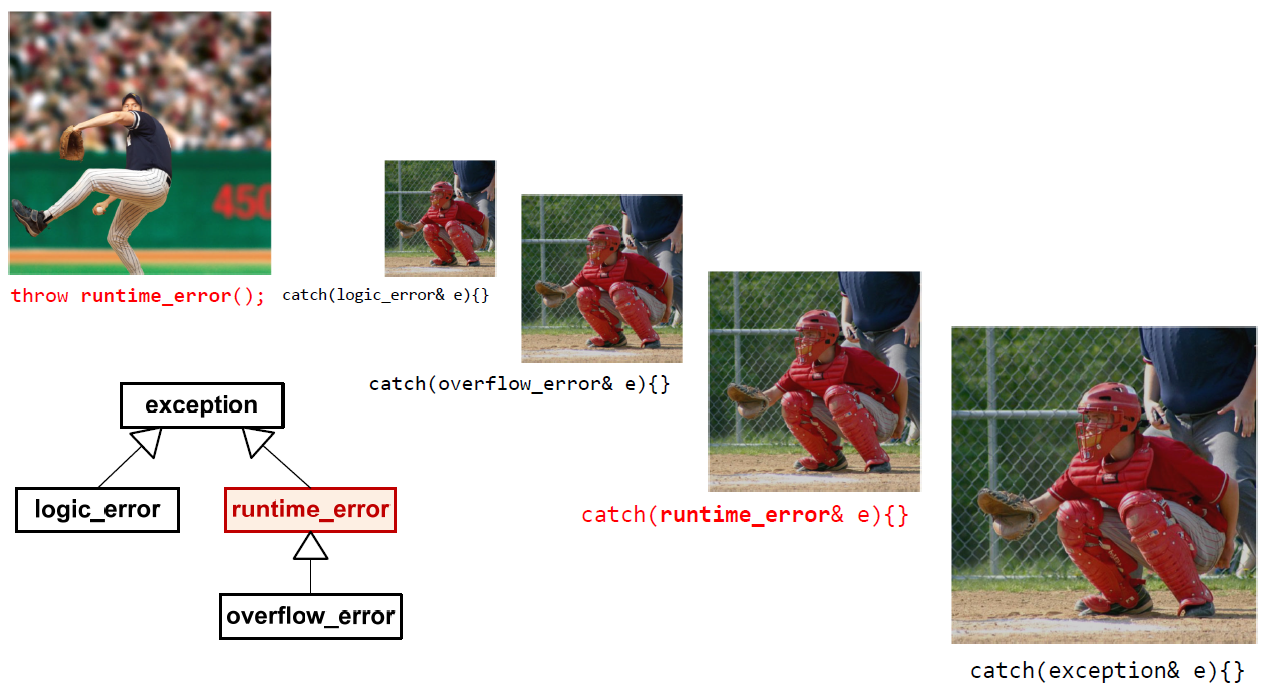
\includegraphics[width=\textwidth]{pics/exceptions.png}
			\end{minipage}
									
		\vspace*{-0.8cm}\paragraph{Exception Specification}
			\lc{void foo() throw(/* Liste der Exceptions */);}
			\begin{compactitem}
				\item Liste beschreibt, welche Exceptions von einem Aufrufer von \lc{foo()} erwartet werden m�ssen.
				\item Aber: garantiert auch, dass das Programm abst�rzt, wenn eine andere als die	spezifizierten Exceptions ausgeworfen wird, d.h. \lc{foo()} muss daf�r sorgen, dass wirklich nur die aufgelisteten Exceptions ausgeworfen werden.
				\item Genauer: falls eine nicht spezifizierte Exception ausgeworfen wird, dann wird die Funktion \lc{unexpected()} aufgerufen, welche �blicherweise das Programm abbricht.
				\item \lc{unexpected()} kann selbst definiert werden.
				\item {\bf Ab \lc{C++11} gilt jedoch:}
				\begin{compactitem}
					\item Exception Specifications sind deprecated (sollen nicht mehr verwendet werden)
					\item Aber: daf�r wurde ein neues Schl�sselwort \lc{noexcept} eingef�hrt, um anzugeben, dass eine Funktion keine
					Exceptions auswirft (na ja)
					\item \lc{noexcept} ist auch ein Operator, dem als Argument ein Funktionspointer �bergeben werden kann
					\begin{compactitem}
						\item returns \lc{true}, falls Funktion mit \lc{noexcept} spezifiziert ist
						\item sonst \lc{false}
					\end{compactitem}
				\end{compactitem}
			\end{compactitem}
	%\end{minipage}
	%\hspace*{0.5cm}
	%\begin{minipage}[t]{10 cm}
		\vspace*{0.2cm}
		{\bf Beispiele:}
		\lstinputlisting{code/exception_specification.cpp}
		{\bf Beispiele ab \lc{C++11}:}
		\lstinputlisting{code/exception_specification_11.cpp}
	%\end{minipage}